\documentclass[conference]{IEEEtran}
\IEEEoverridecommandlockouts
% The preceding line is only needed to identify funding in the first footnote.

\usepackage{cite}
\usepackage{amsmath,amssymb,amsfonts}
\usepackage{algorithmic}
\usepackage{graphicx}
\usepackage{textcomp}
\usepackage{xcolor}
\usepackage{booktabs}
\usepackage{multirow}
\usepackage{url}

\def\BibTeX{{\rm B\kern-.05em{\sc i\kern-.025em b}\kern-.08em
    T\kern-.1667em\lower.7ex\hbox{E}\kern-.125emX}}

% Forces a row break in the \author block (like \and, but starts a new,
% independently centered row) so a 5-author list lays out as 2 / 2 / 1
% instead of letting IEEEtran's automatic wrapping strand the last name.
\makeatletter
\newcommand{\linebreakand}{%
  \end{@IEEEauthorhalign}
  \hfill\mbox{}\par
  \mbox{}\hfill\begin{@IEEEauthorhalign}
}
\makeatother

\newtheorem{remark}{Remark}
\newtheorem{proposition}{Proposition}

\begin{document}

\title{DAB-Guided Weak Supervision and Stain-Shift-Weighted Conformal\\
Prediction for HER2 IHC Intensity Segmentation
\thanks{Funding acknowledgment withheld pending submission.}
}

\author{
\IEEEauthorblockN{J. S. Varughese}
\IEEEauthorblockA{
\textit{Department of Computer Science and Engineering} \\
\textit{Mar Baselios College of Engineering and Technology} \\
Thiruvananthapuram, India \\
johansvarughese.b23cs2135@mbcet.ac.in}
\and
\IEEEauthorblockN{Nadeema Jahan}
\IEEEauthorblockA{
\textit{Department of Computer Science and Engineering} \\
\textit{Mar Baselios College of Engineering and Technology} \\
Thiruvananthapuram, India \\
nadeemajahan.b23cs2146@mbcet.ac.in}
\linebreakand
\IEEEauthorblockN{Aiswarya M S}
\IEEEauthorblockA{
\textit{Department of Computer Science and Engineering} \\
\textit{Mar Baselios College of Engineering and Technology} \\
Thiruvananthapuram, India \\
aiswaryams.b23cs2111@mbcet.ac.in}
\and
\IEEEauthorblockN{Rishika Pratap Jadgale}
\IEEEauthorblockA{
\textit{Department of Computer Science and Engineering} \\
\textit{Mar Baselios College of Engineering and Technology} \\
Thiruvananthapuram, India \\
rishikapratapjagdale.b23cs2155@mbcet.ac.in}
\linebreakand
\IEEEauthorblockN{Dr. Jesna Mohan}
\IEEEauthorblockA{
\textit{Associate Professor, Department of Computer Science and Engineering} \\
\textit{Mar Baselios College of Engineering and Technology} \\
Thiruvananthapuram, India \\
jesna.mohan@mbcet.ac.in}
}

\maketitle

\begin{abstract}
Human epidermal growth factor receptor 2 (HER2) immunohistochemistry (IHC)
scoring assigns breast cancer tissue a 0/1+/2+/3+ membrane-staining
intensity category that determines eligibility for targeted therapy; the
2+ ("equivocal") category triggers a second, costly confirmatory test.
Manual scoring at class boundaries is subjective, and, to our knowledge, no
public dataset provides pixel-level HER2 IHC annotations, so a segmentation
model aimed at this problem has no direct ground truth to train on. We
address this gap with two contributions. First, we train a ResNet18-UNet
segmentation network on pseudo-labels produced by classical DAB
optical-density thresholding, and feed the network that same physically
meaningful DAB channel as a fourth input alongside RGB -- an inductive bias
that lets the model exploit the exact quantity its own weak-supervision
targets are computed from. Evaluated head-to-head against a SegFormer-B0
baseline under identical data, split, seed, and a strict CPU-only compute
budget, this resolves a diagnosed sub-pixel resolution failure: moderate
(2+) intensity segmentation improves from an IoU of 0.00006 (the class is
effectively never predicted) to 0.589, with every other class improving as
well, at roughly three-fold rather than an order-of-magnitude increase in
per-image compute. Second, we generalize an existing image-level, binary
conformal prediction method for HER2 status classification to pixel-level,
five-class segmentation output, and extend it with stain-shift-weighted
calibration for cross-institution robustness. We validate finite-sample
coverage on real held-out data and report the method's honest limits:
calibration against weak-supervision pseudo-labels rather than pathologist
ground truth, and a single-source dataset on which the stain-shift
weighting mechanism is exercised but has nothing genuine to correct. Every
reported number carries the caveats -- weak supervision, no slide-level
split, smoke-scale evaluation -- required to read it correctly; this paper
reports what was actually measured, not what the method aims for once real
multi-institution, pathologist-annotated data exists.
\end{abstract}

\begin{IEEEkeywords}
HER2, immunohistochemistry, weak supervision, semantic segmentation, U-Net,
conformal prediction, uncertainty quantification, digital pathology
\end{IEEEkeywords}

\section{Introduction}

Human epidermal growth factor receptor 2 (HER2) status determines whether a
breast cancer patient is eligible for HER2-targeted therapy. Pathologists
assign a 0/1+/2+/3+ score from the intensity and completeness of membrane
staining on an immunohistochemistry (IHC) slide, following the American
Society of Clinical Oncology / College of American Pathologists (ASCO/CAP)
guideline \cite{wolff2018}. A score of 3+ is positive and 0/1+ is
negative-to-low, but the 2+ ("equivocal") category cannot be resolved from
IHC alone and triggers a second, more expensive confirmatory test
(FISH/ISH). Manual scoring, particularly at the 0-versus-1+ and
2+-versus-3+ boundaries, is known to vary between observers, which
motivates quantitative, AI-assisted pre-scoring tools that reduce that
variability -- not autonomous scoring, but a measurement a pathologist
reviews and confirms.

Building such a tool for HER2 IHC segmentation runs directly into a data
problem that most segmentation literature does not face: \emph{no public
dataset provides pixel-level HER2 IHC annotations}. The publicly available
substitute we use, HER2\_IHC\_40X, provides only one intensity label per
1024$\times$1024 patch and one overall score per source slide -- exactly the
classification-style labels a segmentation model cannot train on directly,
and no slide identifiers at all, which rules out a true slide-level
train/validation split. Any segmentation approach to this problem is
therefore necessarily a \emph{weakly-supervised} one, and the credibility of
every downstream result depends on being explicit about what the model was
actually trained and evaluated against.

A second gap is uncertainty. A pre-scoring tool that hands a pathologist a
single point prediction per pixel, with no indication of when the model is
unsure, invites over-trust at exactly the borderline cases where it matters
most. Conformal prediction offers a distribution-free, finite-sample
coverage guarantee for exactly this purpose, but existing work applying it
to HER2 status operates at image level on a binary positive/negative label
\cite{pintawong2025}, and even the most recent conformal-prediction
treatments of medical image segmentation
\cite{mossina2025,borden2026} are architecture- and task-agnostic
uncertainty wrappers, not calibrated against a weakly-supervised,
ordinal, clinically-defined class structure. A pixel-level, five-class
segmentation output for an ordinal clinical scale needs the method
generalized and re-grounded, not applied as-is.

This paper makes four contributions:

\begin{enumerate}
\item A 4-channel (RGB + DAB optical density) input fusion for a
  ResNet18-UNet that resolves a specific, diagnosed sub-pixel resolution
  failure of a transformer segmentation baseline on the class that decides
  reflex FISH testing.
\item A generalization of image-level, binary conformal HER2
  classification \cite{pintawong2025} to pixel-level, five-class
  segmentation, extended with stain-shift-weighted calibration
  \cite{tibshirani2019} for cross-institution deployment.
\item A head-to-head empirical comparison of two architectures under
  identical data, split, seed, and a strict CPU-only compute budget, with
  the full, honest trajectory reported -- including a smoke-scale result
  that initially pointed the wrong way -- together with a compute/accuracy
  characterization of the trade-off the winning architecture actually buys.
\item A methodological stance, carried through every reported number: each
  result is stated with the caveats required to read it correctly --
  pseudo-label supervision, an inferred rather than verified
  train/validation partition, and a single-source dataset on which the
  stain-shift correction has nothing genuine to demonstrate a benefit
  against -- and we further formalize this weak-supervision setting
  (Section~\ref{sec:formulation}) so the circularity it introduces is
  stated as a property of the estimator, not merely as a caveat in prose.
\end{enumerate}

\section{Related Work}
\label{sec:related}

\textbf{Computational pathology and HER2 IHC scoring automation.} The
broader shift toward AI-assisted diagnosis in digital pathology is
well-documented \cite{bera2019}, and HER2 IHC scoring specifically has
attracted a growing body of automated work. Most of it targets image- or
patch-level classification of the 0/1+/2+/3+ label directly -- recent
examples include pyramid-sampling convolutional architectures for
whole-slide HER2 scoring \cite{selcuk2024} and multi-stage CNN classifiers
for HER2 category prediction \cite{mridha2022} -- rather than pixel-level
segmentation of the staining pattern itself, because pixel-level
pathologist annotation is expensive and, for HER2 IHC specifically, not
publicly available at scale. Our work targets the segmentation problem
these patch-classification approaches sidestep, at the cost of having no
direct pixel-level target to train on.

\textbf{Weak supervision from classification labels.} Where dense
annotations are unavailable, a common strategy in histopathology is to
derive a proxy dense target from a classifier-derived or classical,
inspectable signal and train a segmentation model against it. Multi-layer
pseudo-supervision from patch-level classification labels has been shown
effective for tissue semantic segmentation more broadly
\cite{han2021}, using class-activation-style pseudo-masks as the dense
training target. We follow the same weak-supervision strategy, but our
pseudo-labels are produced by a classical, physically interpretable rule
(DAB optical-density thresholding via colour deconvolution
\cite{ruifrok2001}) rather than by a learned class-activation map, which
keeps the pseudo-label generator itself auditable by a pathologist without
requiring a second trained model to explain the first.

\textbf{Stain variation and normalization.} Colour and intensity variation
across scanners and staining protocols is a well-known confound in
computational pathology; deep generative approaches, including
cycle-consistent adversarial networks for multi-domain stain normalization
\cite{hetz2024}, address it by learning a normalizing transform. We take a
complementary, non-generative approach: rather than transforming images
into a canonical stain space, our stain-shift-weighted conformal predictor
(Section~\ref{sec:conformal-method}) reweights calibration evidence by
estimated stain similarity at inference time, using the same Macenko stain
estimation \cite{macenko2009} (Reinhard normalization \cite{reinhard2001}
is also implemented but unused here, see Section~\ref{sec:preprocessing}).

\textbf{Segmentation architectures.} SegFormer \cite{xie2021} predicts at a
coarse $H/4 \times W/4$ resolution before a final upsample, which is
efficient for natural-image segmentation but, as Section~\ref{sec:diagnosis}
shows, loses exactly the thin structures HER2 membrane staining is made of.
U-Net \cite{ronneberger2015}, with skip connections carrying full-resolution
encoder features into the decoder, is the architecture this failure mode
motivates; we pair it with a pretrained ResNet18 \cite{he2016} encoder.
Focal loss \cite{lin2017} addresses per-pixel class difficulty, complementing
Dice loss's insensitivity to class cardinality on our severely imbalanced
label distribution.

\textbf{Conformal prediction.} Inductive conformal prediction
\cite{vovk2005} produces set-valued predictions with a finite-sample
marginal coverage guarantee, using a nonconformity score and an empirical
calibration quantile. Sadinle et al.\ \cite{sadinle2019} give the
multi-class treatment of the same construction. Tibshirani et al.\
\cite{tibshirani2019} extend conformal prediction to covariate shift via
importance-weighted calibration. Within medical imaging, conformal
prediction has recently been used to wrap U-Net segmentation output with
morphological prediction sets \cite{mossina2025} and to quantify
region-level segmentation uncertainty in clinical workflows
\cite{borden2026}; both are general-purpose, task-agnostic wrappers over an
already-trained segmentation model. Pintawong et al.\ \cite{pintawong2025}
apply inductive conformal prediction with a hinge nonconformity score to
binary, image-level HER2 status classification calibrated against
DISH-confirmed ground truth -- the method we generalize to pixel-level,
five-class segmentation, calibrated against pseudo-labels in the absence of
pathologist ground truth, and extend with a stain-similarity weighting
mechanism specific to the cross-institution deployment setting.

\section{Dataset and the Weak-Supervision Problem}
\label{sec:dataset}

We use HER2\_IHC\_40X, a public patch dataset of approximately 11{,}000
(10{,}997) 1024$\times$1024 RGB IHC patches at 40$\times$ magnification, as
an approved stand-in while a target clinical whole-slide-image dataset
(84 slides, not yet digitized) remains unavailable. Patches are organised
into four folders (\texttt{class\_0}, \texttt{class\_1+}, \texttt{class\_2+},
\texttt{class\_3+}); each patch's filename additionally carries a prefix
naming its source slide's overall score. Cross-tabulating the two labels
over all 10{,}997 patches produces an upper-triangular table -- a patch's
folder-level label is never lower than its slide-level label -- which
establishes that the folder is a finer-grained, patch-level intensity label
and the filename prefix is the coarser slide-level summary. Neither is a
pixel mask. Fig.~\ref{fig:datasetdist} shows the class distribution of the
2{,}200-patch test split used throughout this paper: moderately imbalanced,
with the clinically pivotal moderate (2+) class the rarest at 10\% of
patches.

\begin{figure}[t]
\centering
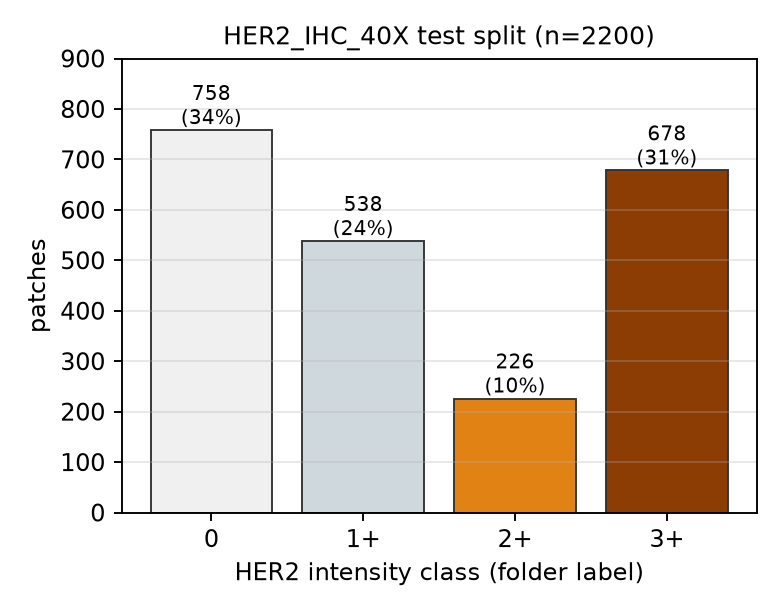
\includegraphics[width=0.8\columnwidth]{../figures/dataset_distribution.png}
\caption{HER2\_IHC\_40X test-split class distribution (folder label).}
\label{fig:datasetdist}
\end{figure}

\textbf{No slide identifiers.} Filenames carry a sparse global counter, not
a slide ID, so the coarsest available grouping is (slide-level score
$\times$ origin token), 8 groups in total, and those groups are confounded
with the label itself: holding out any one group removes an entire
intensity class from training. We therefore cannot construct a true
slide-level split. The held-out set used in this paper is instead defined
by an origin token embedded in each filename, inferred to be the dataset
authors' own train/test assignment -- the dataset's own \texttt{train/} and
\texttt{test/} \emph{directories} were measured to cross this token in both
directions (78\% of files in \texttt{test/} are named \texttt{\_train\_}),
so using the directories directly would have held out a random resample of
the same slides. Table~\ref{tab:splitsizes} gives the resulting sizes. The
validation set is a stratified random draw from the remaining patches and
is explicitly \emph{not} leakage-free; it is used only for epoch selection
and curves, never quoted as a generalization estimate.

\begin{table}[t]
\centering
\caption{Split sizes (source patches; 40$\times$ native tiling produces
4 tiles per patch). Fit/validation are optimistic (not leakage-free);
holdout is the best available approximation to a held-out set on this
dataset.}
\label{tab:splitsizes}
\begin{tabular}{lrr}
\toprule
Split & Source patches & Tiles \\
\midrule
Fit & 200 & 792 \\
Validation & 30 & 119 \\
Holdout (reserved) & 1{,}904 & -- \\
\bottomrule
\end{tabular}
\end{table}

\textbf{Pseudo-labels.} Dense per-pixel targets are produced by thresholding
DAB optical density (Section~\ref{sec:preprocessing}) at fixed cut points
(weak 0.25, moderate 0.50, strong 0.80). We do not treat this as ground
truth uncritically: mean stained tissue area rises monotonically with the
dataset's own patch-level label (Table~\ref{tab:sanity}), at both
20$\times$ and 40$\times$ magnification, which is the expected signature of
a sensible deconvolution and threshold set, and is the only sanity check
available in the absence of real annotations.

\begin{table}[t]
\centering
\caption{Pseudo-label sanity check: mean DAB-thresholded stained-tissue
area rises monotonically with the dataset's own patch label, at two
independently retiled magnifications.}
\label{tab:sanity}
\begin{tabular}{lrr}
\toprule
Folder label & Stained area, 20$\times$ & Stained area, 40$\times$ \\
\midrule
0 & 0.50\% & 0.49\% \\
1+ & 3.84\% & 3.73\% \\
2+ & 22.58\% & 21.47\% \\
3+ & 63.57\% & 62.74\% \\
\bottomrule
\end{tabular}
\end{table}

\textbf{Circularity.} Because the segmentation model trains on these exact
thresholds, a model that agrees with them has demonstrated nothing on its
own. The classical thresholder is carried through every evaluation in this
paper as an experimental control, not discarded once the learned model
exists. Section~\ref{sec:formulation} states this circularity formally.

\section{Method}

\subsection{Problem Formulation and Notation}
\label{sec:formulation}

We make the weak-supervision setting explicit before describing the
pipeline, since every later result inherits its properties from this
setup. Let $x \in \mathbb{R}^{H \times W \times 3}$ denote an RGB patch and
let $y^\star : \Omega \to \{0,1,2,3,4\}$ denote the (unobserved) pixel-wise
map a pathologist would assign over the patch's spatial domain $\Omega$, at
the five intensity levels of Section~\ref{sec:dataset}. No dataset
available to this work observes $y^\star$. Instead, a classical,
deterministic thresholding rule $T_\tau: \mathbb{R}^{H\times W\times 3} \to
\{0,\ldots,4\}^\Omega$, parameterized by fixed DAB optical-density cut
points $\tau = (\tau_1,\tau_2,\tau_3)$ (Section~\ref{sec:preprocessing}),
produces a pseudo-label $\tilde y = T_\tau(x)$ used as a surrogate target.

We train a segmentation network $f_\theta: \mathbb{R}^{H\times W\times 4}
\to \Delta^{4}$ -- mapping a 4-channel (RGB + DAB) input to a per-pixel
categorical distribution over 5 classes, $\Delta^4$ the probability simplex
-- by minimizing an empirical risk with respect to $\tilde y$, not
$y^\star$:
\begin{equation}
\hat\theta = \arg\min_\theta \; \mathbb{E}_{x}\Big[\, \mathcal{L}\big(f_\theta(x),\, T_\tau(x)\big) \Big].
\label{eq:erm}
\end{equation}
\begin{remark}[Circularity]
\label{rem:circularity}
Any statistic computed between $f_{\hat\theta}(x)$ and $\tilde y = T_\tau(x)$
-- including every IoU, Dice, and conformal-coverage number in
Section~\ref{sec:experiments} -- is, by construction of
\eqref{eq:erm}, a measurement of agreement with $T_\tau$, not with
$y^\star$. It upper-bounds neither the model's clinical accuracy nor its
disagreement with a pathologist; it only tells us whether $f_{\hat\theta}$
has learned a spatially coherent, generalizing approximation of a known,
inspectable rule. This is why the classical thresholder $T_\tau$ itself is
retained as an experimental control throughout Section~\ref{sec:experiments}:
without it, an improving IoU against $\tilde y$ is uninterpretable, since it
cannot be distinguished from the model simply memorizing $T_\tau$ more
faithfully.
\end{remark}
This formalizes, rather than merely asserts, why every empirical result
below is reported as agreement with a rule, not as clinical validation --
and it is the reason a genuinely useful next experiment
(Section~\ref{sec:limitations}) is not a larger model or more epochs, but
real pathologist annotations $y^\star$ to replace $\tilde y$ in
\eqref{eq:erm} and in the conformal calibration of
Section~\ref{sec:conformal-method}.

\subsection{Preprocessing}
\label{sec:preprocessing}

HER2 IHC slides are dual-stained: haematoxylin (nuclear counterstain) and
DAB (the HER2 signal). We separate the two with Ruifrok and Johnston colour
deconvolution \cite{ruifrok2001}: pixels are converted to optical density
($OD = -\log_{10}(I/I_0)$), and a $3\times3$ stain matrix (haematoxylin,
DAB, and a residual direction from their cross product) is inverted to
recover per-stain concentration maps. Fig.~\ref{fig:deconv} shows this
decomposition on a real, strongly-stained (3+) patch: the DAB channel
isolates the membrane signal cleanly from the haematoxylin-stained nuclei,
and is the quantity every intensity class and every area percentage in
this paper is ultimately a function of. Stain normalization is implemented
(Macenko \cite{macenko2009}, Reinhard \cite{reinhard2001}) but kept off for
HER2\_IHC\_40X, which is single-source: normalizing would shift the exact
DAB optical densities the classes are defined on, without correcting
anything real.

\begin{figure}[t]
\centering
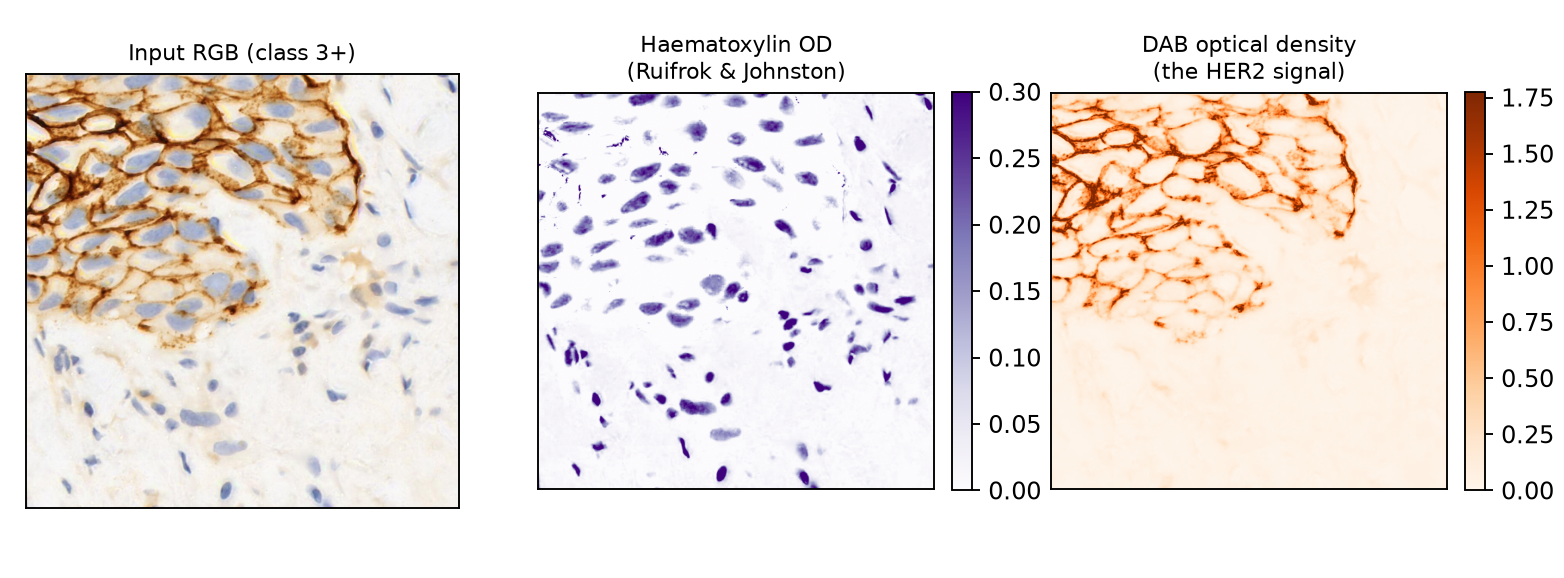
\includegraphics[width=\columnwidth]{../figures/stain_deconvolution.png}
\caption{Ruifrok--Johnston colour deconvolution on a real strongly-stained
(3+) patch: input RGB, recovered haematoxylin channel, and recovered DAB
channel (the HER2 signal every downstream measurement derives from).}
\label{fig:deconv}
\end{figure}

Tissue is detected by mean optical density across RGB rather than by
saturation-based Otsu thresholding: on this dataset, an Otsu threshold on
saturation tracked staining intensity rather than tissue presence (the
chosen threshold rose from $\approx$0.12 on faint patches to $\approx$0.43
on strongly stained ones), silently excluding weakly-stained tissue from
its own denominator. Fig.~\ref{fig:tissue} demonstrates this failure mode
directly on a real faintly-stained patch: the saturation-Otsu mask covers
only 34.9\% of the frame, concentrated on the darkest haematoxylin-stained
nuclei, while the optical-density mask covers 51.9\%, recovering the
faint, diffusely-stained tissue the saturation-based rule discards.
Optical density responds to any stain absorbing light, independent of
which stain or how much.

\begin{figure}[t]
\centering
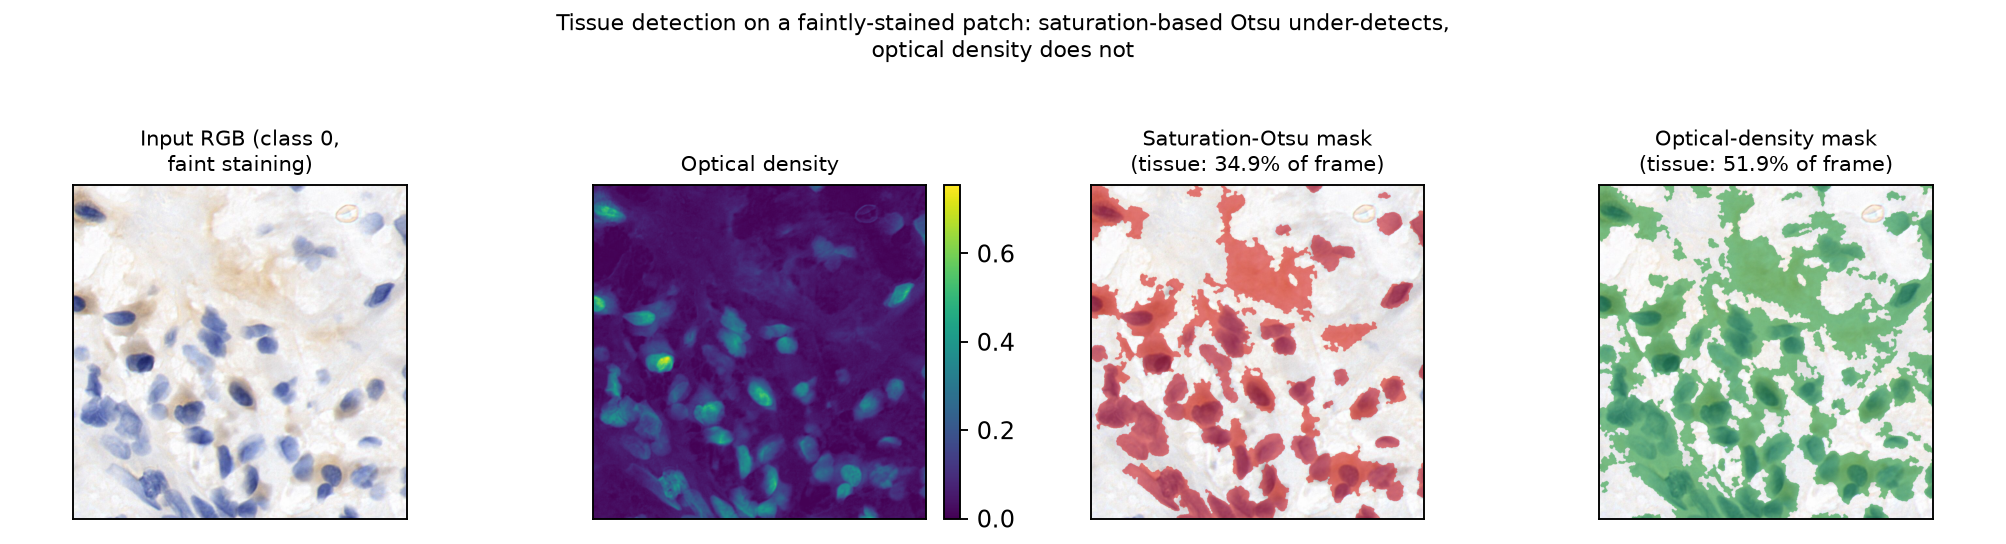
\includegraphics[width=\columnwidth]{../figures/tissue_detection_comparison.png}
\caption{Tissue detection on a real faintly-stained patch. Saturation-based
Otsu thresholding under-detects tissue by discarding weakly-stained regions
from its own denominator (34.9\% vs.\ 51.9\% of the frame); optical-density
thresholding does not have this failure mode.}
\label{fig:tissue}
\end{figure}

Each 1024$\times$1024 patch is tiled into four native-resolution
512$\times$512 tiles (Section~\ref{sec:diagnosis} explains why native
resolution matters), by strided subsampling rather than averaging, which
would blend stained and unstained pixels and shift the optical densities
the classes are defined on. Because the four tiles of one patch are
near-duplicates of each other, the split (Table~\ref{tab:splitsizes}) is
drawn over source patches first and only then expanded to tiles, checked on
every run to guarantee no patch has tiles on both sides of a split.

\subsection{Architecture: ResNet18 Encoder, U-Net Decoder, 4-Channel Input}

Our segmentation network pairs an ImageNet-pretrained ResNet18 encoder
\cite{he2016} with a U-Net decoder \cite{ronneberger2015}. Skip connections
carry the encoder's own full-resolution early feature maps into the
decoder, directly targeting the resolution failure diagnosed in
Section~\ref{sec:diagnosis}, rather than relying on one coarse decode head
and a single upsample to invent detail never actually predicted. A
first version of the decoder ran one additional stage at the input's own
full resolution; measured cost (8 fit / 4 val patches, 1 epoch) was 170
seconds, four times the positions of the stage before it, so the decoder
stops one stage earlier (stride 2, not stride 1) -- still twice
SegFormer's stride-4 output resolution, at a cost this CPU-only machine can
afford. Measured per-image cost (forward + backward, batch size 1, CPU) is
$\approx$4.4\,s, against SegFormer's $\approx$1.45\,s: about $3\times$
slower, not an order of magnitude, for the resolution this architecture
buys back (Fig.~\ref{fig:efficiency} quantifies this trade-off against the
accuracy it purchases).

The network accepts four input channels, not three: RGB plus the DAB
optical-density channel already computed in preprocessing. Because the
pseudo-label targets are themselves a function of DAB optical density, this
hands the model the exact, physically meaningful quantity its own
weak-supervision targets are computed from, rather than requiring it to
re-derive an approximation of DAB absorption from raw RGB through learned
convolutions -- a deliberate inductive bias for a weakly-supervised setting
with very little signal for the rarest class. The first convolution's extra
input channel is initialized from the mean of the pretrained RGB filter
weights, a standard transfer-learning trick for adding a channel without
discarding ImageNet pretraining on the other three. Fig.~\ref{fig:unetarch}
diagrams the full encoder-decoder, including exactly which stride the
decoder stops at and why.

\begin{figure}[t]
\centering
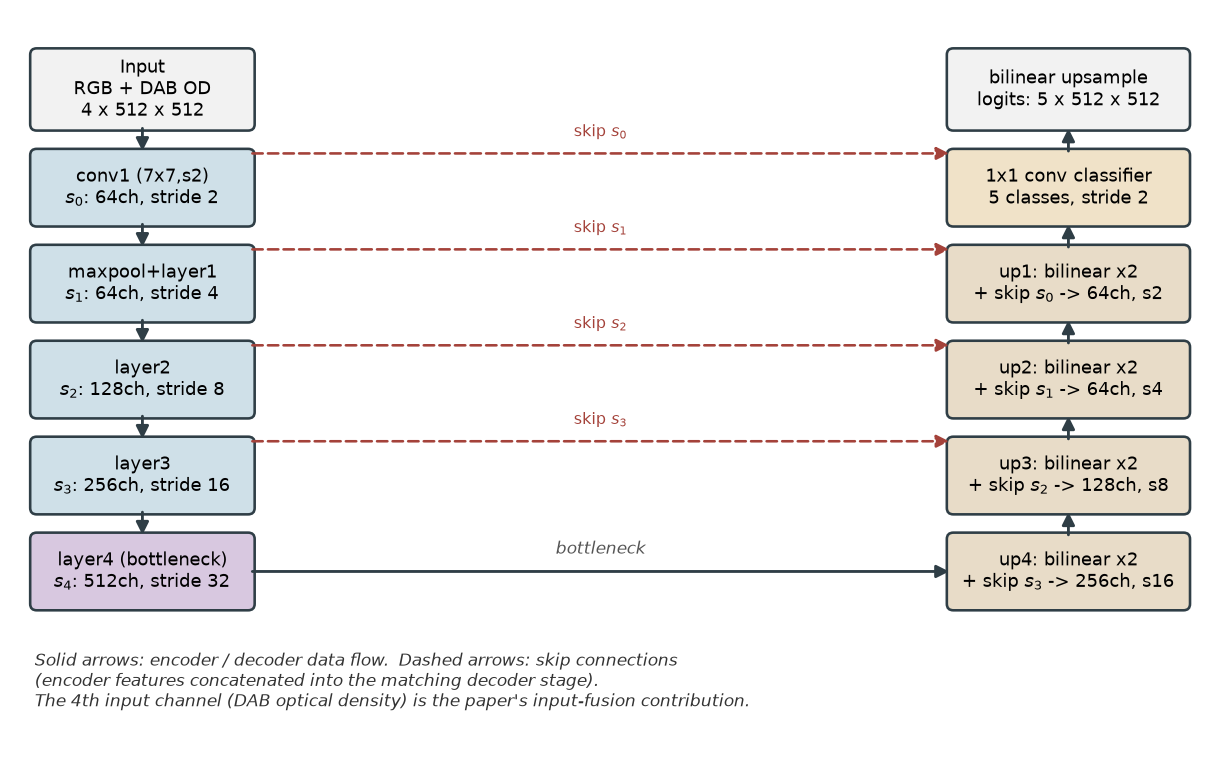
\includegraphics[width=\columnwidth]{../figures/unet_architecture.png}
\caption{ResNet18-UNet architecture, drawn from the model's actual forward
pass. The decoder stops at stride 2 (not stride 1), still twice
SegFormer's stride-4 output resolution, before a final non-learned
bilinear upsample of the logits.}
\label{fig:unetarch}
\end{figure}

\subsection{Loss}
\label{sec:loss}

The class distribution is severely imbalanced at the pixel level
(Fig.~\ref{fig:balance}): background and negative jointly account for
80.8\% of fit-set pixels, while the clinically pivotal moderate (2+) class
is only 3.6\%. We use a weighted sum of cross-entropy (weight 1.0), soft
Dice (weight 0.5, Laplace-smoothed), and focal loss \cite{lin2017} (weight
1.0, $\gamma=2$) to counteract this imbalance from three complementary
angles: cross-entropy is the base likelihood objective; Dice is
insensitive to class cardinality but sensitive to overlap quality; and
focal loss downweights easy, well-classified pixels so gradient from the
rare intensity classes is not drowned out by the two dominant classes.
Dice is averaged only over classes actually present in a given batch --
absent classes are excluded, not scored as 0 or 1, so a patch correctly
containing no strong-staining pixels is not penalized for a class that was
never there.

\begin{figure}[t]
\centering
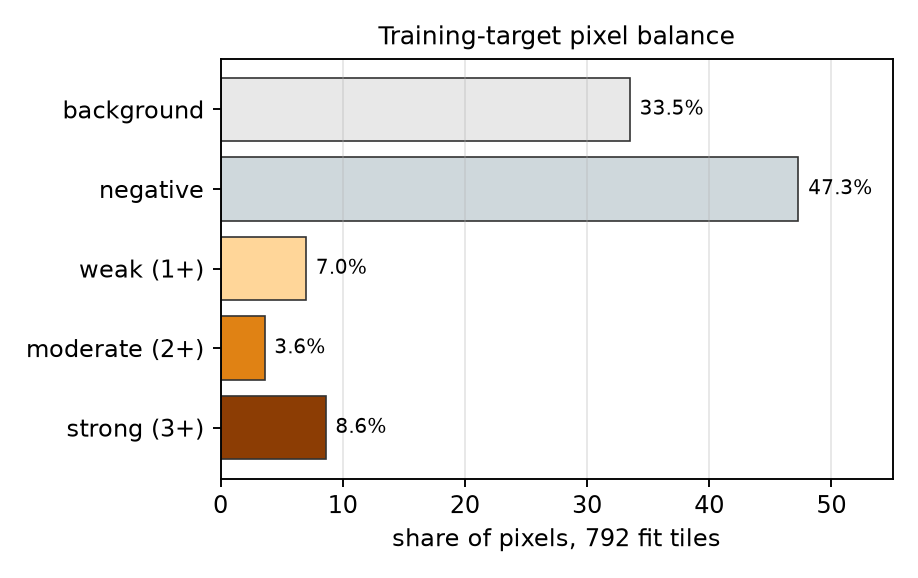
\includegraphics[width=\columnwidth]{../figures/pixel_class_balance.png}
\caption{Pixel-level class balance over the 792 fit-set tiles. Moderate
(2+) is the rarest class by pixel count, not only by patch count
(Fig.~\ref{fig:datasetdist}), which motivates the focal-loss and
inverse-frequency-weighting treatments in Section~\ref{sec:loss}.}
\label{fig:balance}
\end{figure}

Inverse-frequency class weighting is implemented and can be enabled via a
resolved \texttt{"auto"} config value (with a fail-loud guard against
silently training unweighted if resolution is skipped), but a full run
comparing weighted against unweighted training was not completed within
this paper's compute budget; one completed epoch showed a moderate-class
IoU of 0.0849 against 0.0001 at the equivalent unweighted point, which we
report as preliminary evidence that class rarity is a contributing cause,
not as a settled result (Section~\ref{sec:limitations}).

\subsection{The Resolution Diagnosis}
\label{sec:diagnosis}

An initial SegFormer-B0 \cite{xie2021} run at effective 20$\times$
(1024$\times$1024 patches downsampled by 2 into one 512 tile) learned
background, negative and strong staining, but essentially never learned the
two middle classes (weak IoU 0.030, moderate IoU 0.000) despite a healthy
overall pixel accuracy of 0.81 -- a concrete demonstration of why pixel
accuracy is the wrong metric to trust on this task. Qualitative inspection
showed the mechanism: predictions were smooth blobs where the pseudo-label
targets are thin membrane lace. SegFormer's decode head predicts at
$H/4\times W/4$ and is bilinearly upsampled once at the end; at 20$\times$ a
membrane rim is 1--3 pixels wide, sub-pixel at the resolution the model
actually predicts at, before the structure ever reaches the loss.

Retiling each 1024$\times$1024 patch into four \emph{native}-resolution
512$\times$512 tiles, at identical model input size and compute cost,
doubled every membrane's width in pixels. Weak (1+) IoU improved
$11\times$ (0.030 $\to$ 0.341); tellingly, epoch 1 of the native-resolution
run already beat the \emph{entire} four-epoch downsampled run, on 40\% of
the data -- the signature of a resolution problem, not a data-volume
problem. \textbf{Moderate (2+) did not move}: IoU 0.0001, predicted on 253
of 21 million validation pixels. The confusion matrix showed the moderate
row splitting 26\% into weak and 71\% into strong: the model treated the
class as if it did not exist. This is the failure the U-Net decoder and the
4-channel input in this paper directly target.

\subsection{Stain-Shift-Weighted Conformal Prediction}
\label{sec:conformal-method}

We generalize the inductive conformal prediction recipe of Pintawong et
al.\ \cite{pintawong2025} in two directions: from binary to $C=5$ classes,
and from one prediction per image to one prediction per pixel.

\textbf{Nonconformity score.} For a pixel with softmax output $p(x) \in
\mathbb{R}^C$, the hinge nonconformity score for class $c$ is
\begin{equation}
s_c(x) = 1 - p_c(x),
\end{equation}
the direct multi-class generalization \cite{sadinle2019} of the base
paper's binary Eq.~2.

\textbf{Per-class calibration quantile.} For each class $c$, calibration
scores $\{s_c(x_i)\}_{i=1}^{n_c}$ are collected from every calibration pixel
whose pseudo-label is $c$. The unweighted $(1-\alpha)$ quantile is the
standard inductive-conformal empirical quantile \cite{vovk2005},
\begin{equation}
\hat q_c(\alpha) = \left\lceil \frac{(n_c+1)(1-\alpha)}{n_c} \right\rceil\text{-th smallest of } \{s_c(x_i)\},
\end{equation}
which gives the finite-sample marginal coverage guarantee. The
stain-shift-weighted quantile \cite{tibshirani2019} instead assigns each
calibration score a similarity weight
\begin{equation}
w_i = \exp\!\left(-\frac{\lVert d_i - d_{\text{test}} \rVert^2}{2\,h^2}\right),
\end{equation}
where $d_i$ is a 6-dimensional stain descriptor (the haematoxylin and DAB
rows of a per-patch Macenko-estimated stain matrix \cite{macenko2009}) and
$h$ is the median pairwise descriptor distance over the calibration set
(the standard "median trick" bandwidth). Weights are renormalized together
with one reserved unit of weight for the test point itself -- the Gaussian
kernel evaluated at zero distance, so the test point's self-similarity
weight sits on the same scale as every calibration weight rather than an
arbitrary constant -- and the weighted quantile is the smallest score at
which cumulative normalized weight reaches $1-\alpha$. Passing no test
descriptor recovers the unweighted quantile exactly.

\begin{proposition}[Coverage under exchangeability]
\label{prop:coverage}
Under the standard inductive-conformal exchangeability assumption between
the calibration pixels of class $c$ and a test pixel truly of class $c$,
the unweighted prediction set $\{c : s_c(x) \le \hat q_c(\alpha)\}$
contains the true class with probability at least $1-\alpha$, marginally
over the randomness of the calibration draw \cite{vovk2005}. The
stain-shift-weighted variant restores this guarantee under a covariate
shift between calibration and test stain distributions when the weights
$w_i$ correctly approximate the likelihood ratio between them
\cite{tibshirani2019}; Section~\ref{sec:results-conformal} reports the
empirical coverage this proposition predicts, and
Section~\ref{sec:limitations} states plainly that on our single-source
dataset the weighted and unweighted cases are not expected to differ,
since there is no real covariate shift for the weights to correct.
\end{proposition}

\textbf{Prediction sets and patch-level rollup.} A pixel's prediction set
is $\{c : s_c(x) \le \hat q_c(\alpha)\}$. Following the base paper's
image-to-case rollup (their Table~2), each pixel's set reduces to a status
-- a definite class if the set is a singleton, \textsc{ambiguous}
otherwise -- and a patch's status is whichever definite class occupies a
strict majority of its pixels, else \textsc{ambiguous}.

\textbf{What this is calibrated against.} No pathologist pixel annotations
exist anywhere in this project. Calibration uses the same DAB-threshold
pseudo-labels $\tilde y$ of Section~\ref{sec:formulation}. A prediction set
that achieves nominal coverage here has been shown well-calibrated against
$T_\tau$, not against $y^\star$ -- this caveat travels with every conformal
result in this paper, exactly as Remark~\ref{rem:circularity} states for
the segmentation metrics.

\textbf{What is spent, once.} Calibration and evaluation use only the
reserved holdout set (Table~\ref{tab:splitsizes}), split in half into a
calibration set and a test set that never overlap and never touch the
fit/validation data used for model selection.

\section{Experiments}
\label{sec:experiments}

\subsection{Setup}

All experiments run CPU-only (no GPU available), PyTorch, batch size 2 with
gradient accumulation over 4 steps, AdamW at learning rate $10^{-4}$ with
5\% linear warmup, 4 epochs, seed 20260805. The architecture comparison
(Section~\ref{sec:archresults}) uses identical data, split and seed for
both models so the comparison isolates the architecture choice.

\subsection{Architecture Comparison}
\label{sec:archresults}

Table~\ref{tab:archcompare} and Fig.~\ref{fig:archcompare} compare
SegFormer-B0 and our ResNet18-UNet at full scale (200 fit / 30 validation
patches, 4 epochs, identical split and seed). U-Net wins on every class,
most dramatically on moderate (2+): IoU 0.00006 $\to$ 0.589, a result the
smoke-scale run (40 fit / 15 val patches, 3 epochs) did not predict --
at that scale moderate IoU \emph{collapsed} across epochs (0.00022 $\to$
0.00002), which we report because it initially supported the wrong
hypothesis (that the failure was structural to the label distribution,
independent of architecture). The full-scale run reverses that reading:
epoch 1 with 5$\times$ the data already showed non-trivial moderate-class
signal (IoU 0.008), rising to 0.589 by epoch 4. The honest conclusion is
that SegFormer's failure on this class is architecture-specific
(consistent with the $H/4$ resolution diagnosis in
Section~\ref{sec:diagnosis}), not an inherent property of the labels --
but only the full-scale run, not the smoke-scale one, supports that
conclusion, and we report both rather than only the one that agrees with
our hypothesis.

\begin{table}[t]
\centering
\caption{Validation IoU by class, identical data/split/seed, 4 epochs, CPU.
Validation is a stratified random draw from the fit directory, not a
held-out set (see Table~\ref{tab:splitsizes}); numbers are optimistic and
used for architecture comparison, not as a generalization estimate.}
\label{tab:archcompare}
\begin{tabular}{lrrr}
\toprule
Class & SegFormer-B0 & ResNet18-UNet & $\Delta$ \\
\midrule
Background & 0.852 & 0.861 & +0.009 \\
Negative & 0.815 & 0.839 & +0.024 \\
Weak (1+) & 0.341 & 0.666 & +0.325 \\
\textbf{Moderate (2+)} & \textbf{0.00006} & \textbf{0.589} & \textbf{+0.589} \\
Strong (3+) & 0.618 & 0.891 & +0.273 \\
\midrule
Tissue mean IoU & 0.443 & 0.746 & +0.303 \\
Pixel accuracy & 0.862 & 0.908 & +0.046 \\
\bottomrule
\end{tabular}
\end{table}

\begin{figure}[t]
\centering
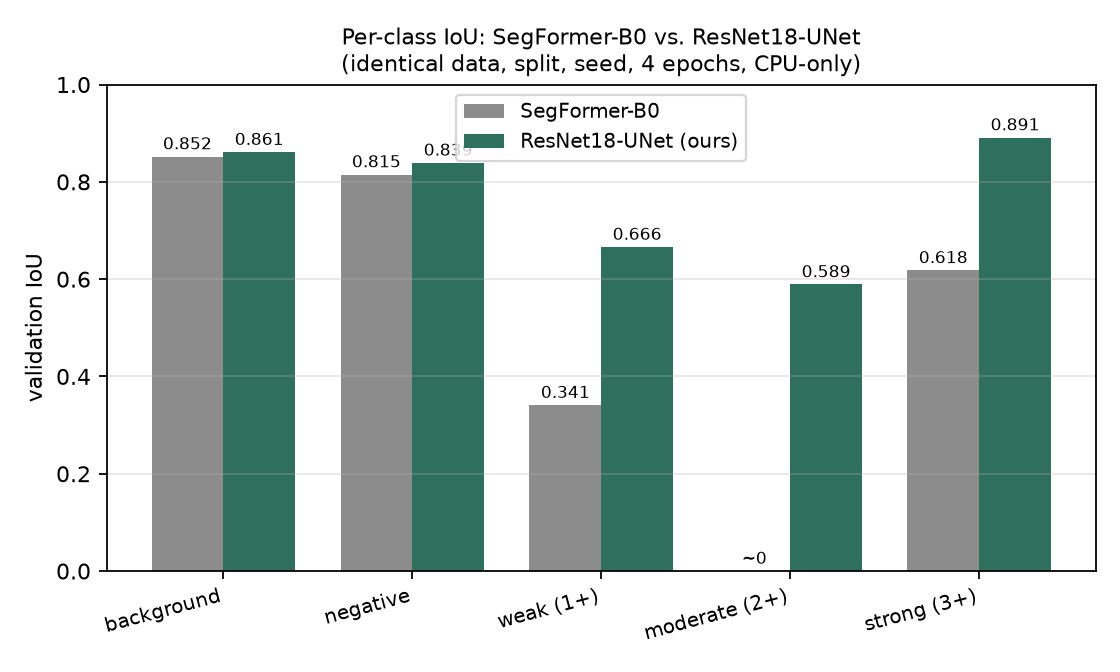
\includegraphics[width=\columnwidth]{../figures/architecture_comparison.png}
\caption{Per-class validation IoU, SegFormer-B0 vs.\ ResNet18-UNet, same
data/split/seed/epochs. Moderate (2+) -- the class that decides reflex
FISH testing -- goes from effectively unlearned to the model's third-best
class.}
\label{fig:archcompare}
\end{figure}

\begin{figure}[t]
\centering
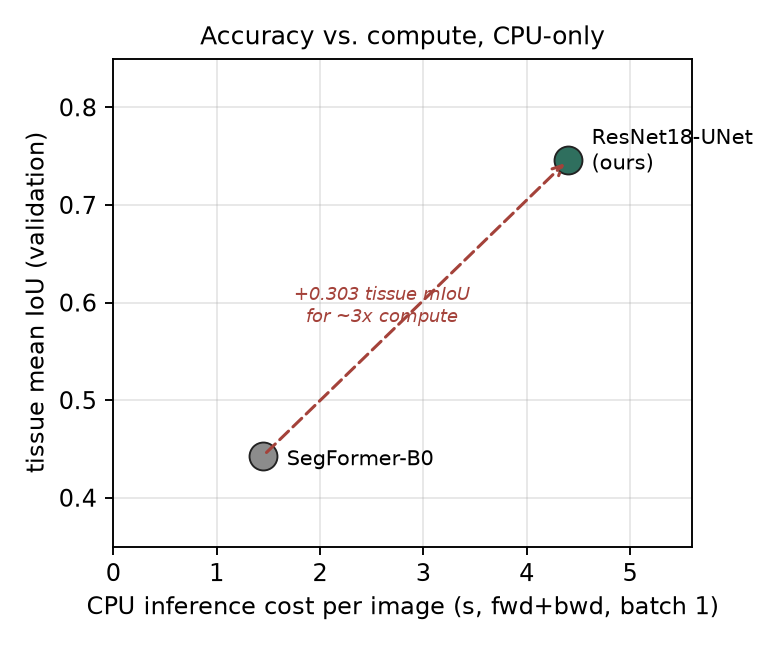
\includegraphics[width=0.92\columnwidth]{../figures/efficiency_accuracy.png}
\caption{The accuracy this architecture buys is not free, but it is cheap:
+0.303 tissue mean IoU for approximately $3\times$, not an order of
magnitude, more CPU inference cost per image.}
\label{fig:efficiency}
\end{figure}

\subsection{Segmentation Results}

Table~\ref{tab:perclass} gives full per-class metrics for the winning
U-Net at its best epoch (4/4, selected on tissue mean IoU). Losses fell
monotonically on both train and validation with no divergence
(Fig.~\ref{fig:training}). Fig.~\ref{fig:confusion} shows the row-normalized
validation confusion matrix: moderate (2+) is still the most-confused
class (12.9\% of its pixels called weak, 11.5\% called strong), but it is
now a real, non-degenerate row rather than an empty one. Fig.~\ref{fig:preview}
shows qualitative predictions against pseudo-label targets across all four
staining intensities, with a per-example pixel-disagreement rate.

\begin{table}[t]
\centering
\caption{Per-class validation metrics, ResNet18-UNet, best epoch (4/4).
Same validation-set caveat as Table~\ref{tab:archcompare}.}
\label{tab:perclass}
\begin{tabular}{lrrrr}
\toprule
Class & IoU & Dice & Precision & Recall \\
\midrule
Background & 0.861 & 0.925 & 0.881 & 0.973 \\
Negative & 0.839 & 0.912 & 0.974 & 0.858 \\
Weak (1+) & 0.666 & 0.799 & 0.710 & 0.915 \\
Moderate (2+) & 0.589 & 0.741 & 0.727 & 0.757 \\
Strong (3+) & 0.891 & 0.942 & 0.950 & 0.935 \\
\midrule
\multicolumn{5}{l}{Tissue mean IoU: 0.746 \quad Pixel accuracy: 0.908} \\
\bottomrule
\end{tabular}
\end{table}

\begin{figure*}[t]
\centering
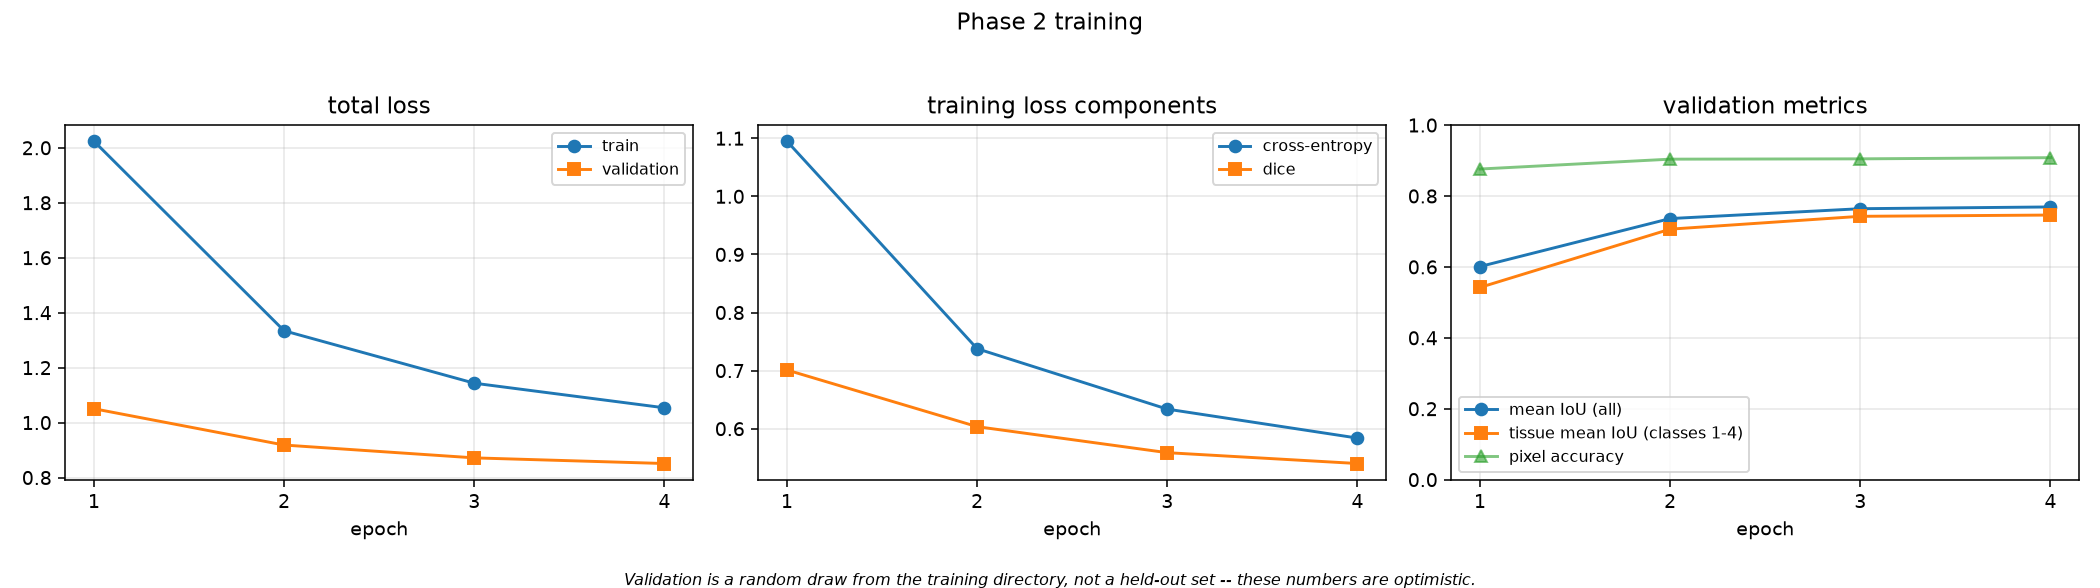
\includegraphics[width=0.95\textwidth]{../figures/unet_training_curves.png}
\caption{Training loss, loss components, and validation metrics across 4
epochs for the winning ResNet18-UNet run. Validation numbers are optimistic
(see Table~\ref{tab:splitsizes}); shown for training diagnostics, not
generalization claims.}
\label{fig:training}
\end{figure*}

\begin{figure}[t]
\centering
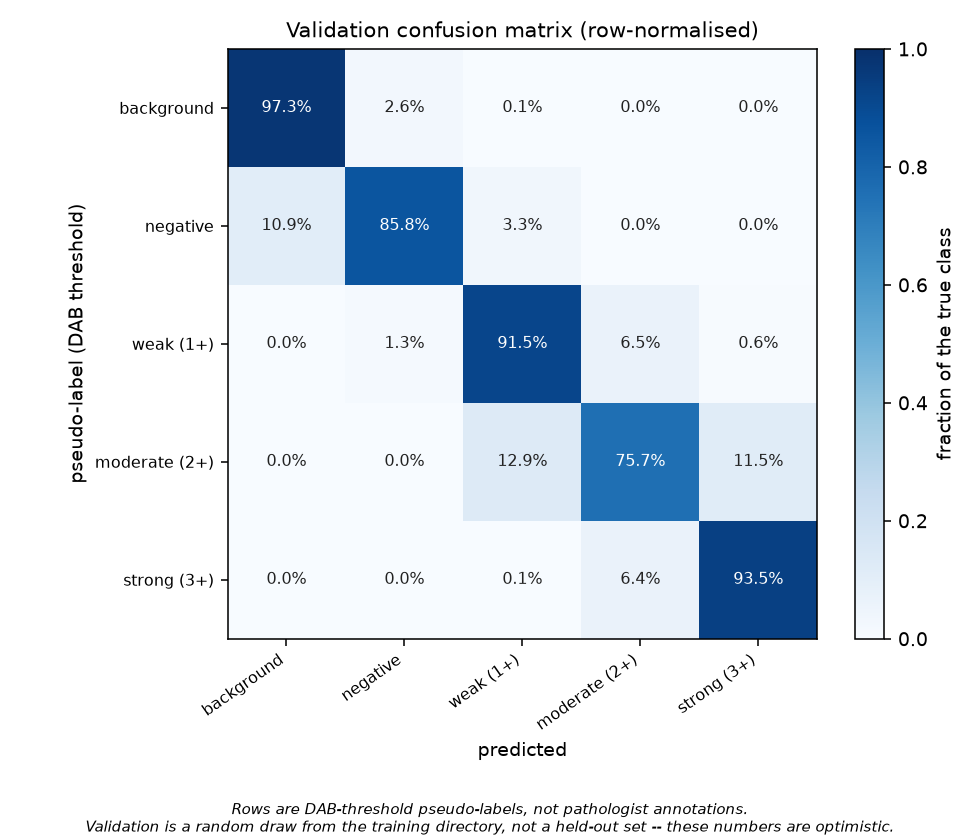
\includegraphics[width=\columnwidth]{../figures/unet_confusion.png}
\caption{Row-normalized validation confusion matrix. Rows are DAB-threshold
pseudo-labels, not pathologist annotations.}
\label{fig:confusion}
\end{figure}

\begin{figure*}[t]
\centering
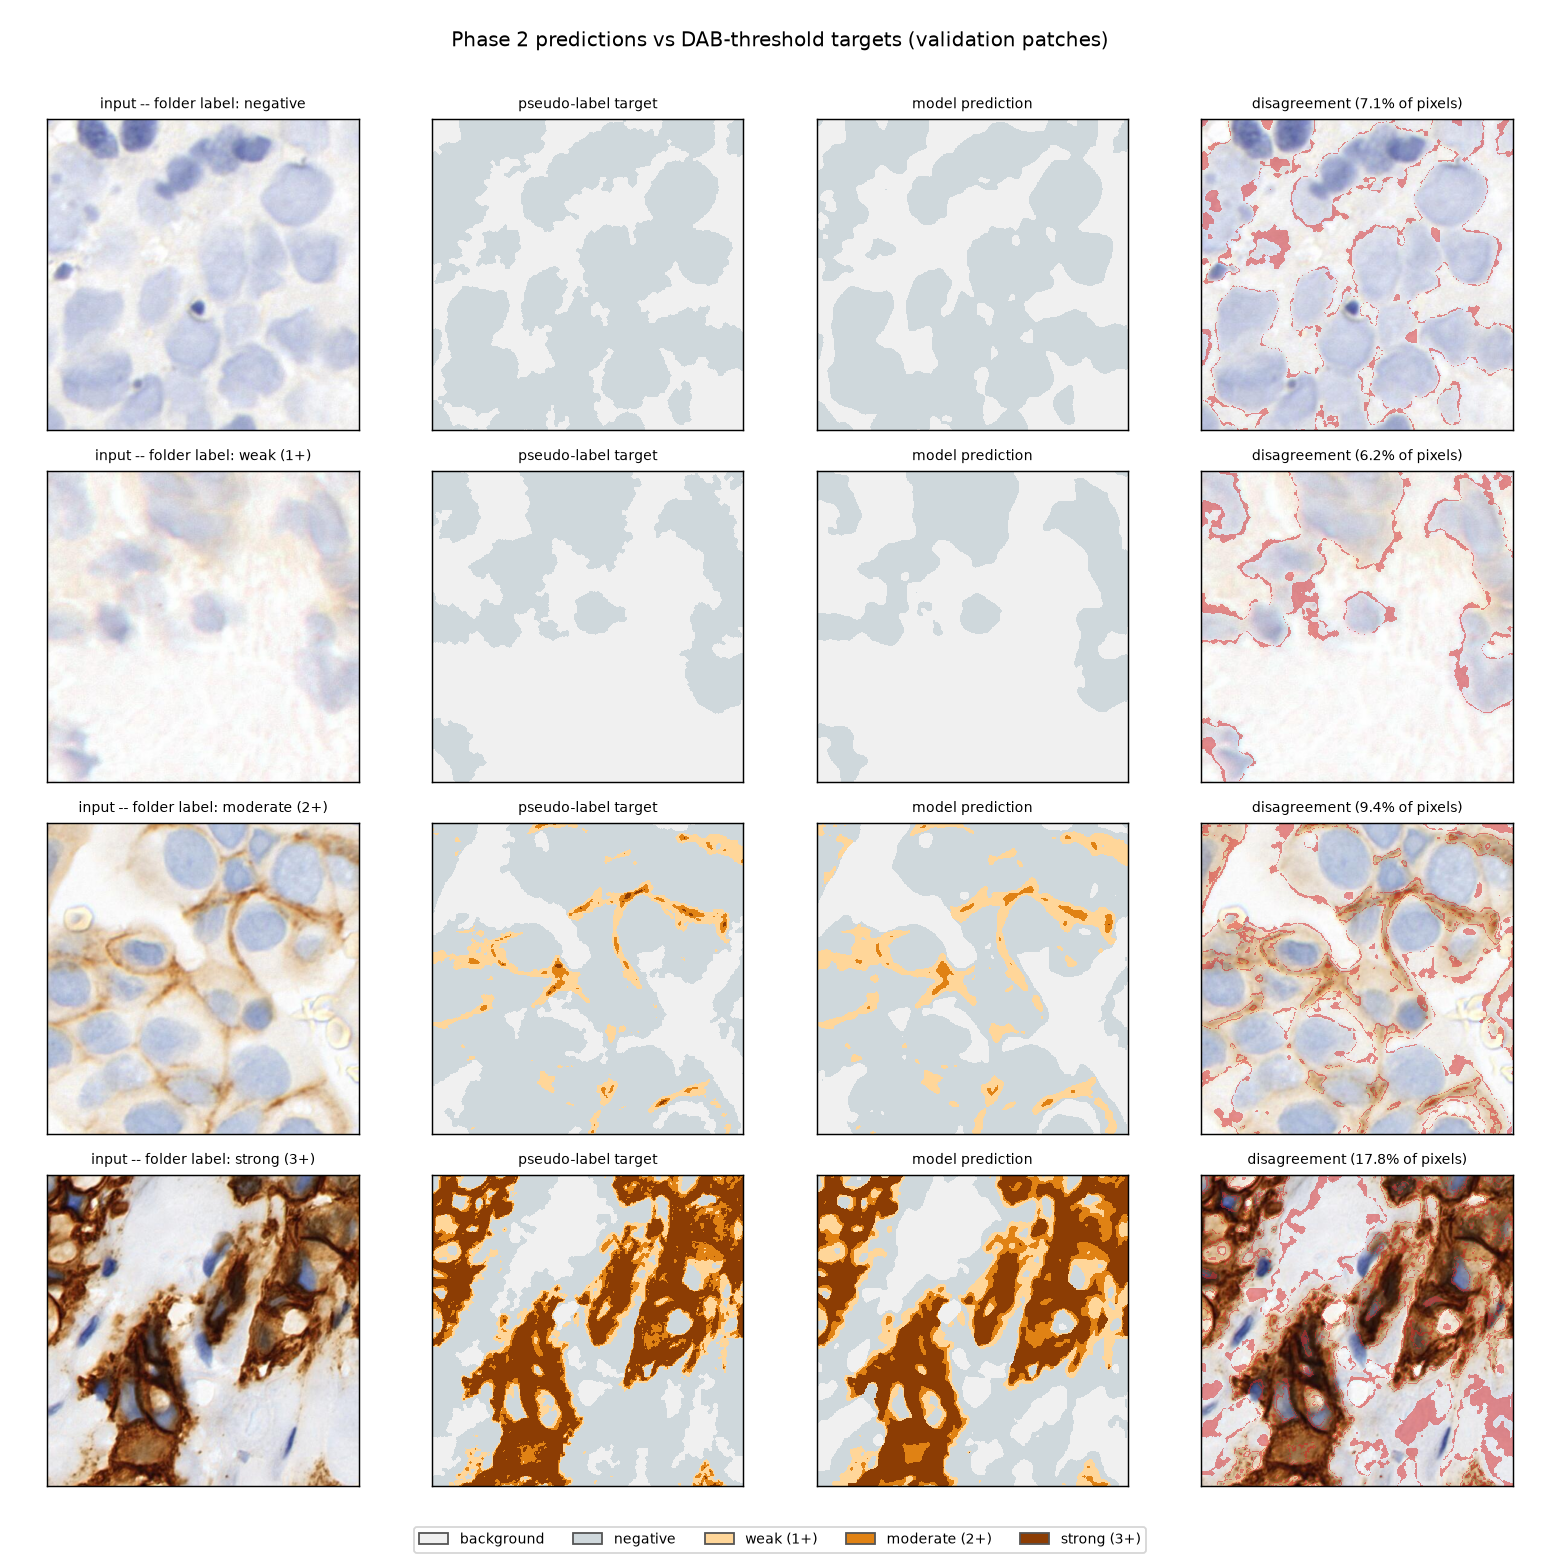
\includegraphics[width=0.95\textwidth]{../figures/unet_prediction_preview.png}
\caption{Input, pseudo-label target, model prediction and pixel
disagreement for one validation patch per intensity class. The model
recovers thin membrane structure the pseudo-label targets are made of,
rather than the smooth-blob failure diagnosed in
Section~\ref{sec:diagnosis}.}
\label{fig:preview}
\end{figure*}

\subsection{Conformal Prediction Results}
\label{sec:results-conformal}

We calibrate and evaluate the method of Section~\ref{sec:conformal-method}
against the winning U-Net checkpoint, using a smoke-scale split of the
reserved holdout set (40 calibration source patches; the corresponding test
half yields 52 held-out tiles, 10{,}595{,}420 tissue pixels). A full-scale
run over the entire $\approx$1{,}900-patch holdout set is software-ready but
unrun -- CPU-only, at the per-tile inference cost measured in
Section~\ref{sec:archresults}, this is a multi-hour job, the same order of
cost as a full training run.

\begin{table}[t]
\centering
\caption{Pixel-level conformal prediction, smoke-scale test set
(52 tiles, 10{,}595{,}420 tissue pixels), calibrated and evaluated against
the winning U-Net checkpoint.}
\label{tab:conformal}
\begin{tabular}{lrrrrrr}
\toprule
& \multicolumn{3}{c}{Unweighted} & \multicolumn{3}{c}{Stain-shift weighted} \\
$\alpha$ & Misc. & Amb. & Acc. & Misc. & Amb. & Acc. \\
\midrule
0.01 & 0.009 & 0.216 & 0.992 & 0.010 & 0.213 & 0.992 \\
0.05 & 0.044 & 0.110 & 0.971 & 0.047 & 0.106 & 0.969 \\
0.10 & 0.089 & 0.072 & 0.950 & 0.093 & 0.072 & 0.949 \\
0.15 & 0.135 & 0.090 & 0.945 & 0.141 & 0.098 & 0.947 \\
0.20 & 0.183 & 0.142 & 0.953 & 0.189 & 0.151 & 0.955 \\
0.30 & 0.282 & 0.258 & 0.967 & 0.288 & 0.265 & 0.969 \\
0.50 & 0.489 & 0.480 & 0.983 & 0.491 & 0.482 & 0.983 \\
\bottomrule
\end{tabular}
\end{table}

\begin{figure*}[t]
\centering
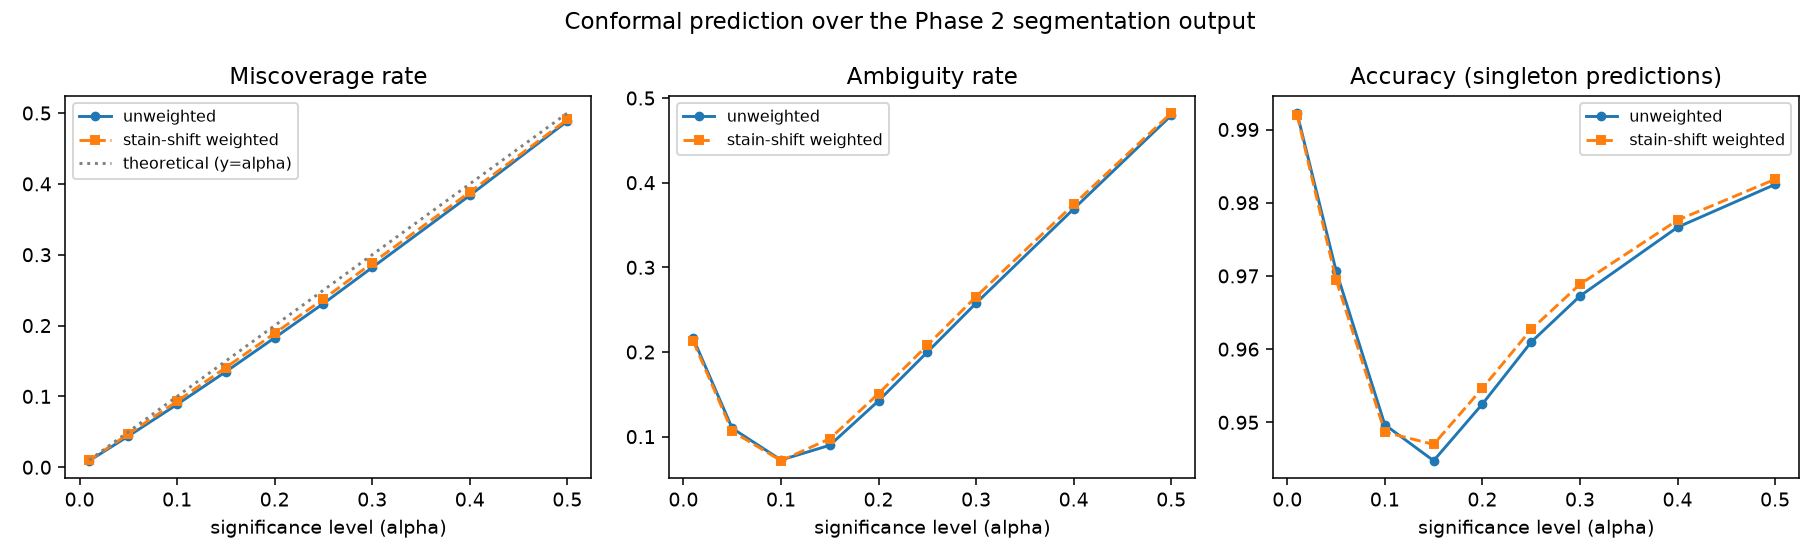
\includegraphics[width=0.95\textwidth]{../figures/unet_conformal_curves.png}
\caption{Miscoverage, ambiguity and singleton accuracy across the
significance-level grid, unweighted vs.\ stain-shift weighted, evaluated
against the winning U-Net checkpoint.}
\label{fig:conformal}
\end{figure*}

Table~\ref{tab:conformal} and Fig.~\ref{fig:conformal} show two things
worth reading directly, exactly as Proposition~\ref{prop:coverage}
predicts. First, \textbf{miscoverage tracks $\alpha$ closely}
(e.g.\ 0.044 at $\alpha=0.05$, 0.089 at $\alpha=0.10$) -- the finite-sample
coverage guarantee holding on real held-out data, the same validation the
base paper's own coverage analysis performs. Second, \textbf{weighted and
unweighted are close at every row}. This is expected, not a failure of the
mechanism: HER2\_IHC\_40X is single-source, so there is no genuine
cross-institution stain shift for the weighting to correct, and
Proposition~\ref{prop:coverage} does not predict a divergence in that
regime. The mechanism itself is validated separately against
deliberately-constructed synthetic multi-source shift in our test suite,
where it measurably favours nearby calibration evidence; on this dataset it
can only be exercised, not shown to help, and we report that honestly
rather than implying a benefit the data cannot demonstrate. Patch-level
accuracy was 1.000 at every $\alpha$ in this run; at 52 test tiles this is
a smoke-sample observation, not a claim about patch-level accuracy at
scale.

\section{Threats to Validity}
\label{sec:limitations}

We organize this section by the standard empirical-software-engineering
taxonomy of validity threats, since a weakly-supervised medical imaging
study has representatives of every category and conflating them obscures
which threats future work can and cannot address by better engineering
alone.

\textbf{Construct validity.} Every reported IoU, Dice, precision, recall
and conformal-coverage number is a measurement of agreement with the
classical DAB-threshold rule $T_\tau$ (Remark~\ref{rem:circularity}), not
with pathologist judgment $y^\star$. This is not a caveat that shrinks with
more data or longer training -- it is definitional to \eqref{eq:erm}, and
only real pixel-level pathologist annotation resolves it. Relatedly,
ASCO/CAP scoring \cite{wolff2018} is defined on percentage of tumour
cells; every measurement here is percentage of tissue area, which
includes stroma, and the two diverge whenever stroma content varies
(mean tissue fraction 0.45 in class 0 to 0.79 in class 3+).

\textbf{Internal validity.} The held-out set in Table~\ref{tab:splitsizes}
is inferred from filename structure, not a verified slide-level partition;
HER2\_IHC\_40X carries no slide identifiers at all. This is the best
available approximation on this dataset, not a leakage-free guarantee, and
it threatens any claim that validation or holdout performance reflects
generalization to unseen \emph{slides} rather than to unseen \emph{patches
of already-seen slides}.

\textbf{External validity.} HER2\_IHC\_40X is single-source. The
stain-shift-weighted conformal predictor is real, unit-tested, and
generalizes correctly on synthetic multi-source shift, but this dataset
offers no genuine cross-institution shift to demonstrate a benefit
against; its practical value is unconfirmed pending real multi-institution
data. More broadly, no claim in this paper should be read as evidence of
performance on the clinical population this project ultimately targets,
whose slides are not yet digitized.

\textbf{Statistical conclusion validity.} The conformal evaluation in
Table~\ref{tab:conformal} is real, computed against the actual deployed
checkpoint, but over 52 of $\approx$1{,}900 available held-out test tiles
-- a full-scale run is software-ready but was not run within this paper's
compute budget. The inverse-frequency class-weighting result in
Section~\ref{sec:loss} is a single completed epoch, reported as
preliminary evidence, not a finished comparison. Neither the architecture
comparison nor the segmentation results are averaged over multiple seeds,
owing to the CPU-only compute budget; single-seed results on a
weakly-supervised target should be read as directional, not as precise
point estimates with implied confidence intervals.

\textbf{The remaining open question.} Moderate (2+) is resolved as
\emph{learnable} (Table~\ref{tab:archcompare}), not as \emph{solved}: at
IoU 0.589 against 0.67--0.89 for the other stained classes, it remains the
weakest class by a real margin, and it is precisely the category that
decides reflex FISH testing. We conjecture, though do not yet test, that
the highest-value next step is not a further architecture search but
reframing 2+ as a per-cell membrane-completeness question rather than a
tissue-area intensity question -- the approach ASCO/CAP itself scores by,
which our pixel-area measurement only approximates.

\section{Broader Impact and Ethical Considerations}

We designed this system around one non-negotiable constraint: it
\emph{measures}, and a pathologist \emph{scores}. Every quantity this
paper reports is an area percentage or a calibrated prediction set, never
a categorical HER2 call, and the surrounding system this method feeds into
enforces that boundary as executable code rather than as a documentation
promise -- an engineering decision motivated directly by the automation-bias
risk that any sufficiently accurate-looking assistive tool for a
high-stakes clinical decision invites over-reliance. Conformal
prediction's role in that design is specifically to make the model's
uncertainty visible rather than to hide it behind a single confident
number; a wide prediction set at a clinically relevant $\alpha$ is a
legitimate, intended output, not a failure mode to be tuned away.

Two further considerations bear directly on responsible deployment. First,
representativeness: HER2\_IHC\_40X's demographic and institutional
provenance is not documented at the level clinical deployment would
require, and every result in this paper should be read as evidence about
this dataset, not as evidence of population-level clinical validity --
this is precisely the gap the stain-shift-weighted conformal machinery of
Section~\ref{sec:conformal-method} is built to eventually address, once
real multi-institution data exists to calibrate it against. Second,
equity of access: by design, every component in this pipeline runs on
CPU-only commodity hardware; a resource-constrained pathology department
without GPU infrastructure is not, on that basis alone, excluded from
using tooling of this kind. We view this as a deliberate, not incidental,
property of the engineering choices in Section~\ref{sec:diagnosis} and
Section~\ref{sec:loss}.

\section{Conclusion and Future Work}

We show that a physically-grounded input channel (DAB optical density,
computed by the same deconvolution the weak-supervision targets derive
from) combined with a resolution-preserving decoder resolves a specific,
diagnosed failure of a transformer segmentation baseline on HER2 IHC's most
clinically consequential class, under a strict CPU-only compute budget. We
further show that an existing binary, image-level conformal prediction
method for HER2 status generalizes cleanly to pixel-level, multi-class
segmentation output, with stain-shift weighting available for
cross-institution deployment once genuinely multi-source data exists to
exercise it. We formalized the weak-supervision setting this all sits
inside (Section~\ref{sec:formulation}) precisely because, on a problem
with no verified slide-level split and no pixel-level ground truth, a
number reported without the estimator properties that produced it is not
reproducible, however precise it looks.

Future work follows directly from Section~\ref{sec:limitations}: a
full-scale conformal evaluation over the entire reserved holdout set; a
completed inverse-frequency class-weighting comparison; multi-seed
replication of the architecture comparison to bound the statistical
conclusion validity threat identified above; real multi-institution data
to genuinely exercise stain-shift weighting; real pathologist pixel
annotations to replace pseudo-label calibration with clinical ground
truth in both \eqref{eq:erm} and Section~\ref{sec:conformal-method}; and a
per-cell membrane-completeness reformulation of the moderate (2+) class,
closer to how ASCO/CAP itself defines the score.

\section*{Acknowledgment}
Acknowledgments withheld pending submission.

\begin{thebibliography}{00}

\bibitem{wolff2018} A. C. Wolff \emph{et al.}, ``Human Epidermal Growth
Factor Receptor 2 Testing in Breast Cancer: ASCO/CAP Clinical Practice
Guideline Focused Update,'' \emph{J. Clin. Oncol.}, vol. 36, no. 20,
pp. 2105--2122, 2018.

\bibitem{pintawong2025} P. Pintawong \emph{et al.}, ``Conformal Prediction
for Uncertainty Quantification and Reliable HER2 Status Classification in
Breast Cancer IHC Images,'' \emph{IEEE Access}, 2025.

\bibitem{mossina2025} L. Mossina and C. Friedrich, ``Conformal Prediction
for Image Segmentation Using Morphological Prediction Sets,'' in
\emph{Proc. MICCAI}, 2025.

\bibitem{borden2026} B. J. Borden, J. B. Graham-Knight, P. Lasserre,
S. Lucas, and R. D. Rajapakshe, ``Uncertainty quantification of U-Net based
segmentation tool using conformal prediction,'' \emph{J. Appl. Clin. Med.
Phys.}, vol. 27, no. 7, p. e70663, 2026.

\bibitem{bera2019} K. Bera, K. A. Schalper, D. L. Rimm, V. Velcheti, and
A. Madabhushi, ``Artificial intelligence in digital pathology -- new tools
for diagnosis and precision oncology,'' \emph{Nat. Rev. Clin. Oncol.},
vol. 16, pp. 703--715, 2019.

\bibitem{selcuk2024} S. Yoruc Selcuk \emph{et al.}, ``Automated HER2
Scoring in Breast Cancer Images Using Deep Learning and Pyramid Sampling,''
\emph{BME Front.}, 2024.

\bibitem{mridha2022} M. F. Mridha, M. K. Morol, M. A. Ali, and M. S. H.
Shovon, ``convoHER2: A Deep Neural Network for Multi-Stage Classification
of HER2 Breast Cancer,'' arXiv:2211.10690, 2022.

\bibitem{han2021} C. Han \emph{et al.}, ``Multi-Layer Pseudo-Supervision
for Histopathology Tissue Semantic Segmentation using Patch-level
Classification Labels,'' arXiv:2110.08048, 2021.

\bibitem{ruifrok2001} A. C. Ruifrok and D. A. Johnston, ``Quantification of
histochemical staining by color deconvolution,'' \emph{Anal. Quant. Cytol.
Histol.}, vol. 23, no. 4, pp. 291--299, 2001.

\bibitem{hetz2024} M. J. Hetz, T. C. Bucher, and T. J. Brinker,
``Multi-domain stain normalization for digital pathology: A
cycle-consistent adversarial network for whole slide images,'' \emph{Med.
Image Anal.}, vol. 94, p. 103149, 2024.

\bibitem{macenko2009} M. Macenko \emph{et al.}, ``A method for normalizing
histology slides for quantitative analysis,'' in \emph{Proc. IEEE Int.
Symp. Biomedical Imaging (ISBI)}, 2009, pp. 1107--1110.

\bibitem{reinhard2001} E. Reinhard, M. Adhikhmin, B. Gooch, and P. Shirley,
``Color transfer between images,'' \emph{IEEE Comput. Graph. Appl.},
vol. 21, no. 5, pp. 34--41, 2001.

\bibitem{ronneberger2015} O. Ronneberger, P. Fischer, and T. Brox, ``U-Net:
Convolutional networks for biomedical image segmentation,'' in \emph{Proc.
MICCAI}, 2015, pp. 234--241.

\bibitem{he2016} K. He, X. Zhang, S. Ren, and J. Sun, ``Deep residual
learning for image recognition,'' in \emph{Proc. IEEE CVPR}, 2016,
pp. 770--778.

\bibitem{xie2021} E. Xie, W. Wang, Z. Yu, A. Anandkumar, J. M. Alvarez, and
P. Luo, ``SegFormer: Simple and efficient design for semantic segmentation
with transformers,'' in \emph{Proc. NeurIPS}, 2021.

\bibitem{lin2017} T.-Y. Lin, P. Goyal, R. Girshick, K. He, and P. Doll\'ar,
``Focal loss for dense object detection,'' in \emph{Proc. IEEE ICCV}, 2017,
pp. 2980--2988.

\bibitem{vovk2005} V. Vovk, A. Gammerman, and G. Shafer, \emph{Algorithmic
Learning in a Random World}. New York, NY, USA: Springer, 2005.

\bibitem{sadinle2019} M. Sadinle, J. Lei, and L. Wasserman, ``Least
ambiguous set-valued classifiers with bounded error levels,'' \emph{J. Am.
Stat. Assoc.}, vol. 114, no. 525, pp. 223--234, 2019.

\bibitem{tibshirani2019} R. J. Tibshirani, R. Foygel Barber, E. Cand\`es,
and A. Ramdas, ``Conformal prediction under covariate shift,'' in
\emph{Proc. NeurIPS}, 2019.

\end{thebibliography}

\end{document}
